\documentclass[a4paper,12pt]{article}
\usepackage[left=2.5cm, top=2cm, right=1.5cm, bottom=2cm]{geometry}

%%% Работа с русским языком
\usepackage{cmap}					% поиск в PDF
\usepackage{mathtext} 				% русские буквы в формулах
\usepackage[T2A]{fontenc}			% кодировка
\usepackage[utf8]{inputenc}			% кодировка исходного текста
\usepackage[english,russian]{babel}	% ло кализация и переносы
%%\usepackage{textcomp}

%%% Дополнительная работа с математикой
\usepackage{amsmath,amsfonts,amssymb,amsthm,mathtools} 
%\usepackage{textcomp}

%% Номера формул
\usepackage{xymtexpdf}
\usepackage{chmst-pdf}

%%% Работа с картинками
\usepackage{graphicx}  % Для вставки рисунков
\usepackage{rotating}
\setlength\fboxsep{3pt} % Отступ рамки \fbox{} от рисунка
\setlength\fboxrule{1pt} % Толщина линий рамки \fbox{}
\usepackage{wrapfig} % Обтекание рисунков текстом

%%% Работа с таблицами
\usepackage{array,tabularx,tabulary,booktabs} % Дополнительная работа с таблицами
\usepackage{longtable}  % Длинные таблицы
\usepackage{multirow} % Слияние строк в таблице


%%% Программирование

%%%tikz
\usepackage{tikz}
\usetikzlibrary{calc}
\usetikzlibrary{patterns}
\usetikzlibrary{shadows}
\usepackage{indentfirst} % Красная строка


\usepackage[os=win, mackeys=symbols]{menukeys}
\usepackage{enumitem}
\usepackage{hyperref}
\usepackage[russian,noabbrev]{cleveref}

\graphicspath{{fig/}{fig2/}}

\usepackage{lastpage}
\usepackage{fancyhdr}


\usepackage{xassoccnt}
\NewTotalDocumentCounter{totalfigures}
\NewTotalDocumentCounter{totaltables}
\NewTotalDocumentCounter{appendixchapters}
\DeclareAssociatedCounters{figure}{totalfigures}
\DeclareAssociatedCounters{table}{totaltables}
\NewTotalDocumentCounter{totalpages}
\NewDocumentCounter{realpages}
\DeclareAssociatedCounters{page}{totalpages}

\makeatletter
\AtBeginDocument{%
	\stepcounter{realpages}%
}
\EveryShipout{%
	\stepcounter{realpages}%
}
\AtEndDocument{%
	\setcounter{xassoccnt@total@totalpages}{\value{realpages}}%
	\write\@auxout{%
		\string\setcounter{xassoccnt@total@totalpages}{\number\value{realpages}}%
	}
}
\makeatother

\usepackage{listings}
\usepackage{color}

\usepackage[toc,page]{appendix}

%%% Заголовок
\author{Ivan Anashkin}
\title{rfbr}
\date{\today}

\begin{document}
\begin{center}
	\textsc{\large{Министерство науки и высшего образования Российской Федерации}\\
	\footnotesize{Федеральное государственное бюджетное образовательное учреждение высшего образования}\\ 
	\small{\textbf{«Казанский национальный исследовательский технологический университет»}}\\}
\end{center}

	\hfill \break
	\normalsize{УДК: 544.272:66.011}\\
	\normalsize{№ Госрегистрации \textbf{АААА-А18-118032690262-8}}\\
	\normalsize{Инв. №}\\
	
	\large
	~\hspace{9cm}\textsc{Утверждаю}
	
	~\hspace{7cm} Проректор по научной работе
	
	~\hspace{7cm}\underline{\hspace{3cm}} Сабирзянов А.Н.
	
	~\hspace{7cm}<<\underline{\hspace{1cm}}>> \underline{\hspace{4cm}} г.
	
	\hfill \break
\begin{center}
	\Large{Отчет о научно~-- исследовательской работе}\\
	\hfill \break
	\Large{по теме: Молекулярно~-- статистическое моделирование процесса ректификации\\(итоговый)}\\
	\hfill \break
	\hfill \break
	\normalsize
	\large
Руководитель темы:\hspace{5cm}   \underline{\hspace{2.7cm}} Анашкин И.П.
\hfill \break
\vspace{8cm}
\hfill \break
 Казань 2020
\end{center}
\thispagestyle{empty} % выключаем отображение номера для этой страницы


\newpage

\section*{Список исполнителей:}
\normalsize{ 
	\begin{tabular}{cccc}
		Руководитель проекта & \hspace{3cm} &  \underline{\hspace{3cm}} & Анашкин И.П. \\\\
		\hfill \break
		Исполнители: &  & \underline{\hspace{3cm}} & Казанцев С.В. \\\\
	\end{tabular}
\thispagestyle{empty} % выключаем отображение номера для этой страницы

\newpage
\section*{Реферат}
страниц -- \TotalValue{totalpages}

рисунков -- \TotalValue{totalfigures}

таблиц -- \TotalValue{totaltables}

приложений -- 1 %\TotalValue{appendixchapters}

Ключевые слова: ректификация, метод Монте-Карло, межмолекулярное взаимодействие
\\

В проекте разработан молекулярно-статистический метод моделирования процесса ректификации. В основе метода лежит комбинация трех подходов: теоретических тарелок, метода Монте~-- Карло и законов сохранения. В основе алгоритма лежит циклическое выполнение следующих этапов: добавление молекул на тарелку питания и удаление молекул из куба колонны и верхней тарелки; расчет фазового равновесия на каждой тарелке; перемещение газовой фазы на тарелку выше, жидкой фазы на тарелку ниже; пересчет энергий и температур на тарелке.

Разработана программа, реализующая основные блоки предложенного алгоритма. Программа написана с использованием программно-аппаратной технологии CUDA, исходный текст программы открыт и размещен в репозитории открытых проектов. Файлы с исходными данными программы совместимы с программным пакетом gromacs. Совместимость форматов позволяет использовать множество созданных ранее файлов с различными наборами параметров межмолекулярного взаимодействия.

Были проведены тестовые расчеты свойств входящих на тарелки потоков на примере модельного флюида, межмолекулярное взаимодействие которого описывается потенциалом Леннард-Джонса. Результаты расчетов совпадают с литературными данными, что свидетельствует о верной работе алгоритма.

Проведены расчеты типовой задачи на компьютерах с различной конфигурацией с целью определения времени расчета.

Создана программа, позволяющая выводить графики с результатами расчетов в виде интернет странички. На данной страничке можно выводить графики зависимость свойств на тарелках по высоте колонны. А также изменения свойств на выбранной тарелке с течением времени, чтобы можно было оценить динамику процесса ректификации.
\thispagestyle{empty}
\newpage

\tableofcontents

\thispagestyle{empty}

\newpage


	
\addcontentsline{toc}{section}{Введение}
\subsection*{Введение}

Ректификация --- один из наиболее распространенных процессов разделения смесей, применяемых в химической промышленности. Для расчета процесса ректификации разработано множество подходов, в основе которых лежит использование данных о фазовом равновесии компонентов разделяемой смеси. Поэтому, расчетную схему ректификационной колонны необходимо дополнить моделями для описания давления насыщенных паров чистых компонентов и коэффициентов активности в смеси. Однако экспериментальные данные доступны не для всех комбинаций веществ, или доступны в ограниченной области состояний. Решением может выступать использование методов групповых составляющих \cite{Skjold-Jorgensen1979,Tiegs1987,Wittig2003}, однако данные методы не гарантируют хорошего согласования с экспериментальными данными.

В данной работе предлагается использование молекулярно-статистических методов для моделирования процесса ректификации. В основе предлагаемого подхода лежит использование законов сохранения, метода теоретических тарелок и метода ансамбля Гиббса для вычисления фазового равновесия.

\section{Молекулярно-статистический метод расчета процесса ректификации}



\subsection{Молекулярно-статистические методы и программные пакеты}

В настоящее время молекулярно~-- статистические методы находят широкое применение в научных исследованиях в различных отраслях. Данные методы позволяют на молекулярном уровне исследовать свойства веществ, а также процессов происходящих на молекулярном уровне. Для проведения моделирования разработано множество пакетов программ, отличающихся функциональностью и условиями предоставления программ \cite{wiki_progs}. Множество программных продуктов создано под коммерческой лицензией, например Material Studio \cite{material_studio} , Materials Science Suite \cite{shedinger} и т.~д. Данные программные продукты нацелены на широкое применение во многих областях, что зачастую плохо сказывается на производительности их вычислений. Однако в них есть свой интерфейс пользователя, что существенно снижает порог вхождения и простоту для конченного потребителя.

Если сравнивать два подхода молекулярного моделирования: метод молекулярной динамики и метод Монте~-- Карло, и их модификации, то наибольшее распространение получил метод молекулярной динамики. В первую очередь это связано с тем, что данный метод позволяет получить кинетические характеристики, такие как коэффициенты диффузии, вязкости и т.~д. Также сравнивая алгоритмы расчета, метод молекулярной динамики позволяет более эффективно использовать параллельные расчеты на нескольких вычислительных ядрах. Данный факт также способствовал большему распространению вычислений с использованием метода молекулярной динамики. Среди программ с открытым исходным кодом можно выделить gromacs \cite{Berendsen1995,Pronk2013,Abraham2015} и LAMMPS \cite{Plimpton1995,Thompson2009} . Данные программы получили широкое распространение за счет открытого исходного кода и большого количества заинтересованных разработчиков, что привело к отличной вычислительной производительности, в том числе на специфическом оборудовании. 

Метод Монте-Карло при моделировании классических (не квантовых систем) также обладает своими преимуществами. Так намного проще реализовано вычисление химического потенциала системы, что позволяет проще производить вычисления фазового равновесия. Так, для вычисления фазового равновесия разработан ансамбль Гиббса \cite{Panagiotopoulos1987,Orkoulas1994}. Среди программного обеспечения с открытым исходным кодом можно выделить towhee \cite{Martin2013}. Данная программа изначально разрабатывалась для моделирования паро~-- жидкостного равновесия и содержит множество наборов параметров для моделирования. Недостатком данного пакета является то, что во времена начала разработки данной программы не были распространены многопроцессорные компьютеры и многоядерные процессоры. Таким образом данный пакет не позволяет в полной мере использовать все достоинства многопоточного вычисления.



\subsection{Многопоточное вычисление и программно-аппаратная технология CUDA}
Использование молекулярно-статистических методов непосредственно связано с развитием вычислительных технологий еще с разработки первых ЭВМ \cite{Allen1988}. Рассматривая развитие персональных компьютеров можно сказать, что увеличение вычислительных мощностей до середины 2000-х годов продолжалось в большей степени за счет наращивания частоты процессора. Однако накладываемые технологические ограничения не позволили превысить номинальную частоту в 4 ГГц для центрального процессора. В 2005 году на рынок выпускают процессор, содержащий два ядра. В дальнейшем происходит тенденция к наращиванию количества ядер в процессоре. Параллельно с этим развиваются программные средства, позволяющие использовать множество потоков для вычисления.

В 2008 году была представлена программно аппаратная технология CUDA использующая для вычислений процессор видеокарты. Отличие от центрального процессора заключается в том, что видеокарта имеет множество специализированных процессоров, их количество в современных видеокартах достигает нескольких тысяч. Данная технология позволяет увеличить производительность для отдельных задач в несколько десятков и сотен раз. Позже появилась аналогичная технология OpenCL, не привязанная к оборудованию конкретного производителя.

В задачах молекулярной динамики использование видеокарт для расчета приводит к увеличению производительности в 10 раз по сравнению с использованием только центрального процессора. Данные технологии реализованы во многих программных продуктах \cite{wiki_progs}.

\subsection{Ансамбль Гиббса} \label{p.gibbs}
Для того чтобы две фазы (обозначенные I и II) находились в равновесии необходимо выполнение следующих условий:
\begin{itemize}
	\item термическое равновесие (равенство температур) $T^I = T^{II}$;
	\item механическое равновесие (равенство давлений) $p^I = p^{II}$;
	\item химическое равновесие (равенство химического потенциала каждого из компонентов) $\mu_i^I = \mu_i^{II}$.
\end{itemize}

Метод ансамбля Гиббса предусматривает моделирование двух ячеек с молекулами, предусматривающие три типа случайных изменений конфигурации:
\begin{itemize}
	\item перемещение молекулы внутри каждой ячейки (перемещение, вращение, изменение внутренней геометрии молекулы);
	\item изменение объемов каждой из ячейки;
	\item перемещение молекул между ячейками.
\end{itemize}
После каждого изменения конфигурации рассчитывается вероятность принятия или отклонения данного изменения. После значительного количества перемещений между двумя ячейками устанавливается равновесие.


\subsection{Алгоритм расчета ректификации}
Согласно предлагаемому методу, ректификационная колонна делится на участки, аналогичные теоретическим тарелкам (теоретическим ступеням). Каждая из тарелок делится на две ячейки, которые соответствуют газовой и жидкой фазам. Суммарный объем газовой и жидкой фазы на каждой из тарелок остается постоянным. С точки зрения конструкции колонны данный указанный суммарный объем характеризует объем колонны между тарелками.При проектировании могут применяться колонны с переменным диаметром, что обеспечивает равномерность газовой фазы по высоте колонны. Таким образом в алгоритме суммарный объем каждой из ячеек может быть задан любой, однако он не меняется во время моделирования.

На тарелке между газовой и жидкой фазами устанавливается фазовое равновесие, рассчитываемое методом ансамбля Гиббса (раздел \ref{p.gibbs}). После достижения фазового равновесия жидкость уходит на нижнюю тарелку, пар поднимается на верхнюю. Молекулы переносят свою энергию (кинетическую и потенциальную) и, исходя из этой энергии, проводится пересчет температуры на новой тарелке. И расчетный цикл повторяется и заново рассчитывается фазовое равновесие. 

Таким образом в колонне можно проследить за материальными (количество молекул каждого из веществ) и тепловыми потоками (энергия молекул). Также в колонне можно выделить внешние материальные и тепловые потоки: приток молекул с исходной смесью, и флегмой, уход молекул с дистиллятом и кубовым остатком.

Блок-схема алгоритма расчета представлена на рисунке \ref{fig:alg_scheme}. На первом этапе проводится чтение исходных данных для моделирования. Далее рассчитываются свойства входящих материальных потоков. При условии, что колонна работает в стационарном режиме, свойства входящих потоков не должны изменяться. И данную процедуру необходимо провести только один раз на начальном этапе. Однако можно предусмотреть динамическое изменение исходного состава. В этом случае вычисление входящих материальных потоков необходимо включить в расчетный цикл.

\begin{figure}
	\begin{center}
		\includegraphics[width=0.5\textwidth]{scheme.png}
	\end{center}
	\caption{Блок-схема алгоритма расчета} \label{fig:alg_scheme}
\end{figure}

Далее рассчитываются внешние материальные потоки (красный блок): добавляется заданное количество молекул на тарелку питания, рассчитывается количество молекул во флегме, а также количество молекул выводимых из куба.

Далее вычисляются условия фазового равновесия на каждой тарелке с использованием ансамбля Гиббса (синий блок).

После установления фазового равновесия на всех тарелках происходит обмен молекулам между тарелками. Жидкая фаза переходит на нижнюю тарелку, газовая фаза переходит на верхнюю тарелку (фиолетовый блок).

На каждую из тарелок можно вводить дополнительные энергетические потоки: подогрев куба колонны, введение дополнительных змеевиков охлаждения и т.д. (зеленый блок)

После перемещения молекул на каждой из тарелок вычисляется температура по внутренней энергии газовой и жидкой фаз (черный блок). Суммарная энергия молекул на тарелке высчитывается как кинетическая и потенциальная энергия молекул газовой и жидкой фаз. Кинетическая энергия может быть вычислена из температуры на тарелке, потенциальная --- как сумма межмолекулярного и внутримолекулярного (потенциал валентных и торсионных углов и т.д.) взаимодействия.
Новая температура на тарелке может быть вычислена из энергии молекул на тарелке с использованием ансамбля с постоянным количеством молекул, объемом и энергией $NVE$ \cite{Lustig1998}.

Альтернативный алгоритм определения температуры основан на на одновременном изменении температуры во время вычисления фазового равновесия. В данном случае блок добавления энергии будет выполнен раньше, чем расчет условий фазового равновесия. Во время вычисления фазового равновесия температура на тарелке будет динамически изменяться таким образом, чтобы на энергия системы была равна сумме энергий поступающих на тарелку молекул с газовой и жидкой фазой, и энергетических потоков. Выбор конкретной из описанных выше  реализаций алгоритма определения температуры будет осуществляться на этапе программирования.
 
Далее алгоритм циклически повторяется до достижения условия стационарности, или любого другого заданного условия. Например при периодической ректификации могут быть задано количество оставшейся жидкости в кубе, при этом будет исследован неравновесный процесс.
 
На рисунке \ref{fig:plate_scheme} представлена схематическое распределение потоков в ректификационной колонне. Цвет стрелок и текста соответствует различным этапам алгоритма, представленного на рисунке \ref{fig:alg_scheme}


\begin{figure}[h]
	\begin{center}
		\includegraphics[width=0.7\textwidth]{column.png}
	\end{center}
	\caption{Схематическое изображение ректификационной колонны (цвет соответствует различным этапам, представленным на рисунке \ref{fig:alg_scheme})} \label{fig:plate_scheme}
\end{figure}

Усреднение свойств смеси на тарелках и выходных потоках (концентрации, температуры, давления и т.д.) проводится после установления стационарности. Достижение стационарности можно отследить по неизменности составов и количества молекул на каждой тарелке.

Достоинства предлагаемого алгоритма расчета:
\begin{itemize}
	\item не нужно заранее знать фазовое равновесие разделяемых компонентов;
	\item расчет ведется с учетом непостоянства мольных потоков по колонне;
	\item возможность исследования как непрерывной так и периодической ректификации;
\end{itemize}
Недостатками является то, что данный метод не учитывает эффективность тарельчатых устройств реальных аппаратов, обусловленной гидродинамической обстановкой. Данную проблему можно решить в будущем.



\section{Программирование}

Хранение данных:
Отдельный массив для координат молекул  Массив[номер тарелки][номер молекулы]
Массив для координат атомов Массив[номер тарелки][номер молекулы][номер атома] --- координаты атомов хранятся относительно центров молекулы. 

массив номеров молекул в жидкости Массив[номер тарелки][максимум молекул]
массив номеров молекул в газе Массив[номер тарелки][максимум молекул]

\subsection{Перемещение из жидкости в газ или наоборот}
\begin{itemize}
	\item Выбираем случайную молекулу
	\item Рассчитываем энергию в текущем объеме
	\item Выбираем случайные координаты в другом объеме и рассчитываем энергию
	\item При успешном переносе молекулы за место текущего индекса подставляем последний и уменьшаем количество молекул на одну
	\item новые координаты вставляем в конец массива и добавляем количество молекул
\end{itemize}

\subsection{Перемещение молекулы в текущем объеме}
Изменяем только координаты в массиве молекулы

\subsection{Вращение молекулы}
При вращении изменяется только координаты в массиве для атомов
\section{Алгоритм вычисления свойств компонентов на тарелках}

На рисунке \ref{fig:algo1} представлен алгоритм работы программы. На данном рисунке не показан первый этап связанный с расчетом энергии молекул добавляемых в систему. Часть алгоритма, выполняемая на видеокарте выделена прямоугольником. Как показали исследования наилучшим оказался альтернативный вариант, в котором происходит варьирование температуры для достижения заданного значения энергии на тарелке.

\begin{figure}
	\begin{center}
		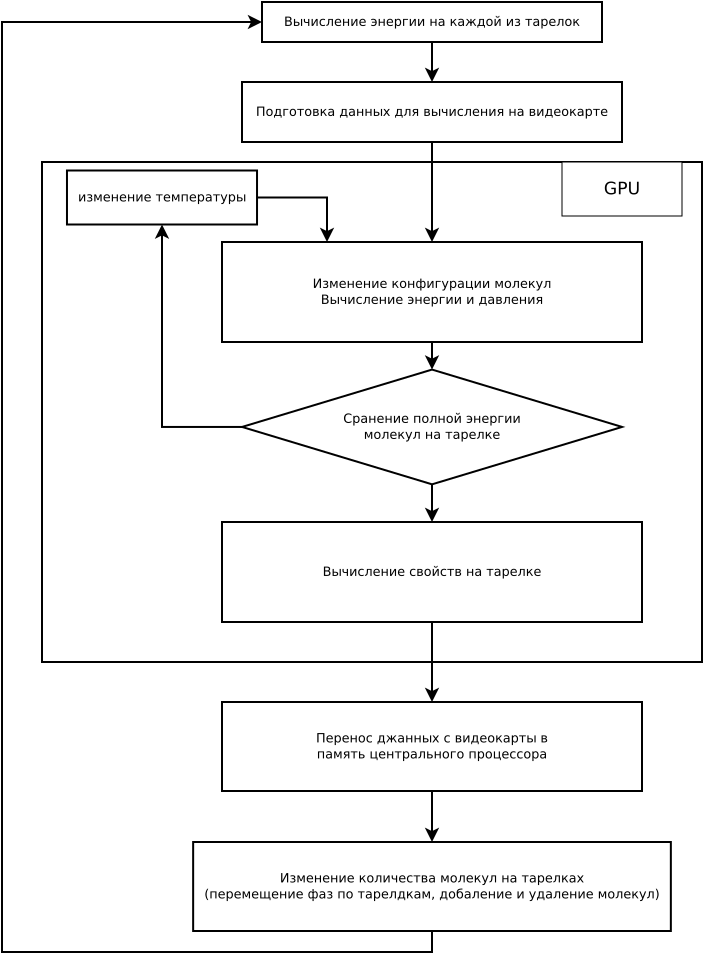
\includegraphics[width=0.5\textwidth]{algo1.pdf}
	\end{center}
	\caption{Алгоритм расчета свойств на тарелках} \label{fig:algo1}
\end{figure}

На первом этапе исходя из вычислений свойств входящих потоков определяется значение энергии, которое необходимо добавляется с входящим потоком:
\begin{equation} \label{eq:inen}
	E_{in} = E_K + E_P = \dfrac{3}{2} k_B T \sum_{i=1}^{I} N_i  + \sum_{i=1}^{I} E_i  N_i  
\end{equation}
где $E_{in}$ --- энергия молекулы с входящим потоком; $E_K$ --- кинетическая энергия; $E_P$ --- потенциальная энергия; $k_B$ --- константа Больцмана; $T$ --- температура; $N_i$ --- количество молекул типа $i$; $E_i$ --- энергия одной молекулы, вычисленная на предыдущем этапе, $I$ --- количество добавляемых в ячейку молекул.

Далее необходимо из энергетического баланса определить суммарную (референсную) энергию на тарелке:
\begin{equation}
	E_{ref} = E_{in} + E{l} + E{v} - E_{loss}
\end{equation}
определяемую как сумма входящих потоков ($E_{in}$) в случае тарелки питания, энергии жидкости ($E_l$) преступаемой с верхней тарелки,  и энергии паровой фазы ($E_v$) с нижней тарелки, ($E_{loss}$) --- потеря энергии за счет теплообмена с окружающей средой (на данный момент данный функционал не реализован). Энергия жидкости и пара может быть вычислена по выражению \eqref{eq:inen}. В случае, если в колонне нет молекул, то энергия складывается только из энергии поступающих на тарелку питания молекул.

Первичная конфигурация молекул реализована в исходном файле <<dbox\_init.cu>>. Заданное в файле конфигурации программы количество молекул расставляется случайным образом в узлах кубической кристаллической решетки. 

\subsection{Алгоритм вычисления на видеокартах}

При моделировании методами молекулярной динамки и Монте ~-- Карло, система ведет себя макроскопически если в ней содержатся несколько сотен молекул. Однако с увеличением количества молекул увеличивается точность расчета за счет двух факторов. Во-первых размер системы ограничивает радиус обрезания потенциала, а он с вою очередь влияет на рассчитанные термодинамические и кинетические свойства \cite{Moultos2016,Jamali2018}. Во-вторых при увеличении размера системы уменьшаются флуктуации свойств в рассматриваемой ячейке, что позволяет уменьшать статистическую ошибку определения.

В настоящее время для высокопроизводительных расчетов широко применяются видеокарты. Графические процессоры по сравнению с центральными процессорами имеют на 2 порядка большее количество ядер, так новое поколение видеокарт Nvidia имеют более 1000 CUDA ядер. Однако для эффективного использования ресурсов необходимо программировать на достаточно низком уровне: вручную выделять и освобождать память, хранить 2 экземпляра переменных на центральном и графическом процессоре отдельно. Также в отличии от центрального процессора, графические процессоры имеют несколько типов памяти регистровая, текстурная, общая.

В описанном выше алгоритме большую часть времени исполнения занимает вычисление свойств фаз на тарелках. Данные вычисления на каждой тарелке являются независимыми, поэтому могут быть проведены параллельно без потери производительности. Вычисление свойств входящих потоков проводилось на одной видеокарте (с индексом 0), в связи с тем, что обычно ходящий поток обычно один. Однако количество тарелок в реальных колоннах обычно больше 5, поэтому было принято решение использовать все доступные в системе видеокарты для увеличения производительности. В настоящее время использую дополнительно оборудование возможно одно временное использование вплоть до 16 видеокарт на одном компьютере.

\subsubsection{Представление данных в памяти видеокарты}

В памяти центрального процессора координаты молекул и атомов представлены в виде многомерных массивов. Размер массива определяется уровнем рассматриваемой абстракции. Свойства тарелок (например энергия, вириал, давление и т.д.) хранятся в одномерном массиве, индекс которого соответствует номеру тарелки. Свойства молекулы (координаты, текущая внутренняя и внешняя энергия и т.д.) представляют из себя двумерный массив, первый индекс которого соответствует номеру тарелки, второй --- номеру молекулы на тарелке. По аналогии с предыдущими примерами для свойств атома (координаты) массив трехмерный, последний индекс которого соответствует номеру атома в молекуле.

Однако указанную структуру данных нельзя использовать в видеокартах. Данные в памяти видеокарты могут быть представлены в виде одно или двумерного массива. Поэтому в данной работе описанная структура данных, преобразовывать которую удобно, преобразовывалась а одномерные массивы для расчета свойств фаз на тарелках. Структура данных представлена на рисунке \ref{fig:data_sheme}.

\begin{figure}
	\begin{center}
		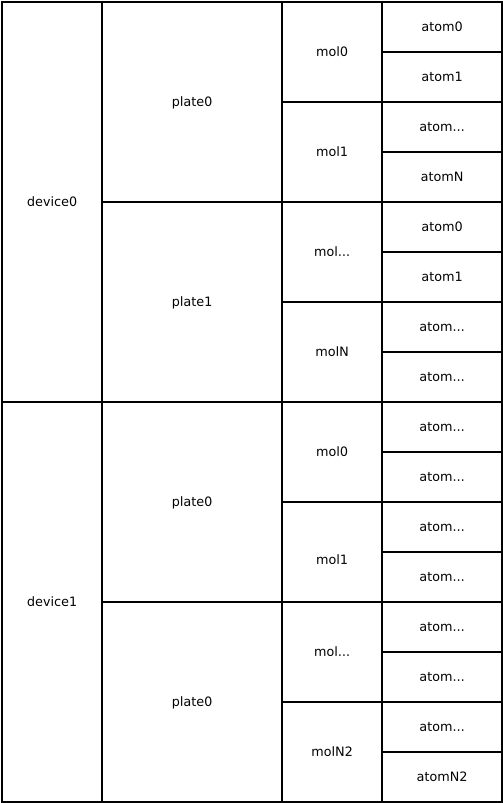
\includegraphics[width=0.5\textwidth]{data.pdf}
	\end{center}
	\caption{Представление данных в памяти видеокарты} \label{fig:data_sheme}
\end{figure}

Расчеты каждой из тарелок осуществляются различными видеокартами (указаны на рисунке как <<device0>> и  <<device1>>). Количество молекул во все колонне может быть очень большое, поэтому для уменьшения времени копирования из памяти центрального процессора в память видеокарты каждая видеокарта получает лишь набор данных который будет обрабатывать. Все молекулы и атомы обрабатываемых тарелок на каждой из видеокарт хранятся в одном массиве. Поэтому для того, чтобы определять к какой тарелке относится та или иная молекула, был создан отдельный массив хранящий индекс первой молекулы на тарелке. Остальные молекулы на тарелке отсчитываются относительно данного индекса. Аналогичная ситуация с атомами, в памяти видеокарты хранится массив с индексом первого атома в каждой молекуле. Подготовка данных и копирование данных из памяти центрального процессора на видеокарту реализован в фале <<double\_devtohost.cu>>.

\subsubsection{Изменение конфигурации молекул}

Вычисление фазового равновесия системы предполагает как минимум у типа изменения конфигурации молекул: перемещение молекул, изменение объемов паровой и жидкой фаз и перенос молекул между фазами. В каждом из типов изменения системы необходимо рассчитать  энергию системы до и после изменения конфигурации. Принятие или не принятие данного перемещения рассчитывается по вероятности исходя из разницы энергии системы и температуры. Таким образом выстраивается марковская цепь, описывающая эволюцию рассматриваемой системы в фазовом пространстве. 

Вычисление энергии системы является одной из наиболее затратных операций, потому что необходимо вычислить потенциал взаимодействия одной молекулы со всеми соседями. В связи с тем, что координаты молекул не меняются во время расчета энергии системы, данная операция проводилась во множество потоков:
\begin{itemize}
	\item Каждый поток вычисляет энергию взаимодействия с $N_{mol}/N_{thread}$ молекул, где $N_{mol}$ ---количество молекул, $N_{thread}$ --- количество потоков. Таким образом каждый поток рассчитывает взаимодействие с определенной частью молекул и записывает энергию в отдельный элемент массива.
	\item Для того, чтобы убедиться, что все энергии были подсчитаны проводится барьерная синхронизация.
	\item Далее проводится суммирование элементов массива с использованием одного из алгоритмов адаптированных для видеокарт \cite{cudabook}.
\end{itemize}

При перемещении молекулы вероятность принятия перемещения определяется выражением \cite{Fernandes2015}:
\begin{equation}
	p_{move} = exp \left(\dfrac{-(U_{new} - U_{old})}{k_B T} \right)
\end{equation}
где индексы $new$ и $old$ показывают новое и старое состояние системы. Если энергия в новой конфигурации системы меньше чем в старой, то данное перемещение примется (вероятность равна 1).

Аналогичные выражения записываются для изменения объема газовой и жидкой фаз:
\begin{equation}
	p_{vol} =  exp \left(\dfrac{-(U_{new.vap} + U_{new.liq} - U_{old_vap} - U_{old.liq})}{k_B T} 
	- N_{vap} \ln \left( \dfrac{V_{vap} + \Delta V}{V_{vap}} \right) \\
	-  N_{liq} \ln \left( \dfrac{V_{liq} - \Delta V}{V_{liq}} \right) 
	\right) 
\end{equation}
где $vap$ и $liq$ --- индексы показывают энергию газовой и жидкой фазы, $\Delta V$ --- изменение объема системы, $N_{vap}$ и  $N_{liq}$ --- количество молекул в газовой и жидкой фазе.

Вероятность перемещения молекулы из одной фазы в другую:
\begin{equation}
p_{vol} =  exp \left(\dfrac{-(U_{new.vap} + U_{new.liq} - U_{old_vap} - U_{old.liq})}{k_B T} 
- \ln \left( \dfrac{V_{vap} (N_{liq})}{V_{vap}} \right) \right) 
\end{equation}

Указанные типы изменения конфигурации системы реализованы в разработанной программе. На каждом шагу Монте-Карло происходит случайное перемещение молекулы. Каждый 10 шаг в значения энергии, давления, количества молекул, объема, плотности записываются в переменную для усреднения. Каждый 100 шаг происходит попытка изменения объема газовой и жидкой фаз, а также перемещения случайной молекулы между фазами.

Изменения (расстояние перемещения молекулы, изменение объема) проводятся на случайную величину. Максимальное значение перемещения динамически изменяется каждые 10000 попыток перемещения таким образом, чтобы отношение приятных к непринятых  перемещений было примерно равно 0.5. Для этого при увеличении отношения более 0.6 шаг увеличивается на 20\%. Аналогично при снижении отношения менее 0.4, шаг уменьшается на 20 \%. Также шаг не может превышать половину длины ячейки и быть меньше 0.01 нм. Максимальное изменение объема жидкой фазы фиксировано и составляет 1\%.

\subsubsection{Определение температуры на тарелках}

Для вычисления температуры на тарелке, необходимо, чтобы рассматриваемая система находилась в равновесии. Для определения достижения равновесия, вычисления разбиваются на блоки (на момент отладки программы размер блока составлял 100000 шагов Монте~-Карло). В каждом из блоков определяются средние значения свойств (энергии, давления, плотности, концентрации и т.д.). 

Для того, чтобы определить, установилось ли равновесие в системе, определяется среднее значение по 5 последним блокам. Равновесие считается достигнутым, в том случае, если отклонения от среднего значения составляют более 5\% (проценты отличаются для каждого из свойств).
Проверка установления осуществляется по следующим свойствам: по энергии паровой и жидкой фаз, плотности жидкой фазы, давлению паровой фазы.
Давление жидкой фазы и плотность газовой испытывают большие флуктуации, поэтому по этим величинам сложно оценивать достижение равновесия системы.

После установления равновесия определяется энергия молекул на тарелке как сумма энергий газовой и жидкой фазы, а также кинетической энергией:
\begin{equation} \label{eq:curen}
E_{cur} = \dfrac{3}{2} k_B T (\sum_{i=1}^{N_{vap}} + \sum_{i=1}^{N_{liq}}) + E_{vap} + E_{liq}
\end{equation}

Далее осуществляется сравнение энергии $E_{cur}$  с рефересной энергией $E_{ref}$. К случае, если текущая энергия системы больше, то температура системы снижается (и наоборот в случае если энергия меньше) и цикл повторяется. В случае если разница энергий не превышает 2\%, то далее проводится дополнительный расчет, с большим количеством перемещений большей статистики в усреднении свойств системы.

\subsection{Перенос молекул между тарелками}

После установления равновесия происходит перенос молекул газовой фазы на одну тарелку вверх, молекулы жидкости на одну тарелку вверх, а также добавление или удаление молекул. Для экономии занимаемой оперативной памяти на видеокарте память на каждую тарелку выделяется согласно количеству молекул. Поэтому для изменения количества молекул на тарелке необходимо пересоздать массивы с новым количеством молекул и данная процедура должна проводиться на центральном процессоре.


\subsection{Влияние гидродинамической обстановки на процесс переноса}

Предложенный алгоритм не учитывает гидродинамическую обстановку на тарелке. Количество молекул в рассматриваемых системах не позволяет каким либо образом учитывать конструкцию тарелок. Разработанный метод также ка и метод теоретических тарелок основан на том, что на тарелке происходит установление термодинамического равновесия. Несмотря на это можно предложить два варианта которые в дальнейшем можно реализовать для решения данной проблемы.

Первый вариант основан использовании полуэмпирических выражений для определения к.п.д. по Мерфи. Для расчета данных коэффициентов необходимы коэффициенты переноса (диффузии, вязкости). Поэтому конфигурацию молекул, вычисленную в а разработанной программе можно использовать для расчета коэффициентов переноса с использованием пакета gromacs. При этому вычисления условий равновесия и коэффициентов переноса можно проводить параллельно.

Второй вариант основан на том чтобы не дожидаться установления условий равновесия на тарелке. Тогда состав, плотности и другие свойства на тарелке будут зависеть от количества сделанных шагов Монте~-Карло. Количество шагов Монте-Карло изоморфно времени в методе молекулярной динамики. Таким образом регулируя количество шагов изменяется время взаимодействия пара и жидкости. 


\subsection{Окружение и установка}

Сборка приложения осуществляется с использованием пакета Cmake, набора компиляторов gcc и библиотек cuda toolkit установить которые можно командой:
\begin{lstlisting}
sudo apt install cmake
sudo apt install gcc g++
sudo apt install nvidia-cuda-toolkit 
\end{lstlisting}

Для выявления зависимостей и создания файлов сборки необходимо запустить команду:
\begin{lstlisting}
cmake
\end{lstlisting}
Различные версии cuda toolkit обычно совместимы не с последней версией gcc, поэтому при компиляции можно указать какую именно версию компилятора использовать:
\begin{lstlisting}
cmake -DCMAKE_C_COMPILER=/usr/bin/gcc-6 -DCMAKE_CXX_COMPILER=/usr/bin/g++-6
\end{lstlisting}
Далее необходимо скомпилировать программу с помощью команды:
\begin{lstlisting}
make
\end{lstlisting}
В папке появится исполняемый файл.

\section{Визуализация расчетов программы}

Молекулярно-статистические методы требуют существенных вычислительных затрат. В связи с этим даже на высокопроизводительном оборудовании время, затраченное на вычисления, может составлять десятки часов. При моделировании неравновесных или неустановившихся процессов необходимо контролировать текущее состояние системы. В большинстве случаев программы сохраняют текущие свойства в виде текстовых файлов, например такие программы как gromacs \cite{Pronk2013} и towhee \cite{Martin2013}. Для визуализации данных можно воспользоваться графическими редакторами. Однако данный способ требует затрат времени. 

Программа осуществляет запись физико-химических свойств паровой и жидкой фаз на каждой тарелке ректификационной колонны в файл. Для каждой тарелки создается папка с названием <<plate-№тарелки>>, в котором хранятся результаты расчетов. Энергия, давление и другие 
Первая строка файла содержит описание характеристики, вторая строка содержит размерность величин. Последующие строки содержат значения физико-химических величин. 
Пример файла с данными:
\lstset{language=Pascal}
\begin{lstlisting}
cycle number	energy	vapor composition	pressure	temperature
no	J/mol	mol frac	bar	K
1	120	0.2	1	260
2	135	0.3	1.32	270
3	136	0.4	1.5	300
4	144.78803861562	0.556133765765478	2.3	310.10013627195
5	144.169386641327	0.5985991615124	3.16980857747587	310.555670976329
6	149.548525999929	0.501446874120906	3.16782959526555	310.003258276753
7	143.827119599023	0.585662135528444	3.16576977542854	310.944407476643
8	144.044716862953	0.599590463074216	3.08448201449308	310.329150103861
9	140.981959721285	0.527323214848039	3.02232150777213	310.080746716385
10	142.261477555272	0.548889975154957	3.11709420795045	310.003285864423
11	142.70898377206	0.564050477341758	3.01853174591303	310.968434813629
12	148.736902128591	0.575276156796512	3.18153658794448	310.839816872137
13	142.534306535427	0.548514678067799	3.19647971887008	310.119976620409
14	146.832988894578	0.537850383551013	3.15039582146607	310.32992897198
15	147.334992635238	0.54314051251355	3.05684519392893	310.266979312755
16	148.508113161646	0.563352449814567	3.12608646490167	310.692168231217
17	140.378344446634	0.521147735449389	3.16522065313047	310.773110326238
18	143.936391754645	0.502328285553782	3.13219699869719	310.167883000741
19	145.145474369276	0.564324288088821	3.18101680540676	310.174601223762
20	143.089074971632	0.572295830897665	3.06052441556237	310.761356159448
\end{lstlisting}

Визуализация расчетов реализована в виде интерактивной веб-страницы с возможностью выбора нужных параметров для отрисовки графиков. Обработка пользовательских запросов, парсинг данных и подготовка их для визуализации реализована на бэкенде веб-приложения, написанного на языке Python с фреймворком Flask \cite{flask}, непосредственно отрисовка графиков выполняется в браузере пользователя посредством фреймворка highcharts.js \cite{highcharts} языка программирования javascript.
Веб-приложение можно запускать как из непосредственно рабочей папки с расчетами, так и просто имея сохраненные выходные данные программы, в таком формате можно стартовать его как из-под Linux, так и из-под Windows или MacOS. Также можно настроить доступ к визуализации расчетов не только с локальной машины, на которой запущен веб-сервер, но и из внешнего интернета, настроив проксирующий веб-сервер, например, nginx.
На графики независимо друг от друга может выводиться статистика в двух срезах (рисунок \ref{fig:site}): термодинамический параметр на определенной тарелке в динамике всех циклов или термодинамический параметр в определенном цикле по каждой тарелке.

\begin{figure}
	\begin{center}
		\includegraphics[width=0.8\textwidth]{site.png}
	\end{center}
	\caption{Интерфейс веб-страницы с выводом данных в виде графика зависимости состава пара от цикла моделирования и зависимость состава пара на тарелках для заданного цикла моделирования} \label{fig:site}
\end{figure}

Количество тарелок / циклов / термодинамических параметров для визуализации высчитывается независимо от пользователя на основе парсинга визуализируемых данных. Таким образом, можно применять веб-интерфейс для контроля промежуточных результатов эксперимента без дополнительных настроек. Это позволяет осуществлять оперативный контроль результата моделирования, отслеживать момент установления термодинамического равновесия и проводить анализ результатов.

\subsection{Установка программы визуализации}

Установка и настройка программы визуализации проходит следующим образом:
\begin{itemize}
	\item Необходимо установить python и venv с подошью команд
	\begin{lstlisting}
	sudo apt install python3
	sudo apt install python3-venv
	\end{lstlisting}
	\item Программу можно склонировать из github репозитория:
	\begin{lstlisting}
	git clone https://github.com/kzncvs/mc_visualisation.git
	\end{lstlisting}
	\item Переходим в папку с программой:
	\begin{lstlisting}
	cd mc\_visualisation
	\end{lstlisting}
	\item Создаём виртуальное окружение
	\begin{lstlisting}
	python3 -m venv venv
	\end{lstlisting}
	\item Применяем виртуальное окружение
	\begin{lstlisting}
	source venv/bin/activate
	\end{lstlisting}
	\item Устанавливаем зависимости
	\begin{lstlisting}
	pip install -r requirements.txt
	\end{lstlisting}
	\item  Запускаем веб-сервер
	\begin{lstlisting}
	python3 app.py --host=127.0.0.1 --port 5000
	\end{lstlisting}
	\item Папка с исходными данными задается в фале  DATASET\_FOLDER/app.py
	
	
	Сайт с графиками доступен по адресу 127.0.0.1:5000.
	
\end{itemize}



\addcontentsline{toc}{section}{Заключение}
\section*{Заключение}
В работе предложен метод расчета процесса ректификации с использованием молекулярно-статистических методов. Метод базируется на следующих допущениях:
\begin{enumerate}
	\item количество молекул на тарелке рассчитывается исходя их входящих на тарелку потоков жидкой фазы с верхней тарелки, и газовой фазы нижней тарелки;
	\item на тарелку питания и с верхней и нижней тарелки добавляется и удаляются заданные количество молекул;
	\item суммарная энергия молекул на тарелке высчитывается исходя из материальных потоков пунктов 1 и 2;
	\item можно задавать дополнительный подвод (например в кубе колонны) или отвод энергии;
	\item на тарелках устанавливаются условия фазового равновесия, рассчитываемые методом Монте-Карло с использованием ансамбля Гиббса, температура и соответствующие условия равновесия определяются рассчитанной полной энергией молекул на тарелке.
\end{enumerate}

Таким образом соблюдаются законы сохранения массы и энергии. Достоинством описанного метода является то, что для расчета процесса ректификации нет необходимости в экспериментальных или полуэмпирических (выражений коэффициентов активностей и давления насыщенных паров чистых компонентов) данных по условиям фазового равновесия. Метод позволяет рассчитывать периодические и непрерывные процессы с различным количеством входящих и выходящих потоков как массы так и энергии.

Разработанный алгоритм расчета частично реализован в виде программы. Для увеличения производительности программы использована программно-аппаратная технология CUDA, позволяющая проводить вычисления на графических процессорах. Исходный код программы выложен в репозитории github (ссылка https://github.com/MonteCarloRect/mcrec) под открытой лицензией. Сравнение энергии и давления для входящих на тарелку питания потоков леннадж-джонсовского флюида с литературными данными показало хорошее согласование данных. Это свидетельствует о верной реализации алгоритмов молекулярного моделирования.

В связи с тем, что для увеличения производительности программы программа разрабатывалась с возможностью использования всех установленных на компьютере видеокарт, написание и отладка программы существенно усложнилась. Поэтому не хватило времени для реализации блока переноса молекул между тарелками. На начало работы над проектом литературный обзор показал, что нет программ позволяющих вычислять фазовое равновесие с использованием метода ансамбля Гиббса на видеокартах. Это послужило одной из причин написания программы заново, а не использование готового кода. В настоящее время уже существуют программы с открытым исходным кодом, позволяющие рассчитывать фазовое равновесие молекулярными методами на видеокартах \cite{Nejahi2019}.Использование кусков кода данной программы может ускорить разработку. 


Для визуализации расчетов создана программа (ссылка на репозиторий \\ https://github.com/kzncvs/mc\_visualisation)позволяющая на web-станице в интерактивном режиме просматривать результаты расчетов в виде графиков зависимости свойств по высоте колонны и в зависимости от цикла работы программы. 

%\newpage
\addcontentsline{toc}{section}{\bibname}
\bibliographystyle{utf8gost71u}  
\bibliography{lib.bib}
\appendix
\section{Приложение}
% the \\ insures the section title is centered below the phrase: AppendixA

Файлы проекта с описанием содержания (представлены только основные файлы проекта):
\begin{itemize}
	\item build --- тестовая сборка для отладки
	\begin{itemize}
		\item A.gro --- файл координат атомов в молекуле
		\item data.mcr --- файл с параметрами моделирования
		\item B.gro  --- файл координат атомов в молекуле 
		\item data.top --- файл топологии молекул
		
	\end{itemize}
	\item doc --- документация по проекту
	\item initial --- моделирование входящих потоков
	\begin{itemize}
		\item data\_from\_device.cu --- перенос данных из видеокарты в хост
		\item device\_prop.cu --- определение свойств видеокарты
		\item initial\_flows.cu --- задание начальной конфигурации молекул во входящем потоке
		\item read\_gro.cu  --- чтение gro файлов
		\item read\_top.cu --- чтение top файлов
		\item data\_to\_device.cu 	--- перенос данных из хоста в видеокарту
		\item free\_arrays.cu --- освобождение памяти на видеокарте
		\item rcut.cu --- вычисление добавки, связанной с обрезанием потенциала взаимодействия
		\item read\_options.cu --- чтение параметров моделирования из файла 
		\item single\_box.cu --- основной алгоритм метода Монте-Карло
	\end{itemize}
	\item write --- содержит файлы с выводом логов и выходных данных
	\item CMakeLists.txt --- конфигурация для сборки Cmake
	\item global.h --- глобальные константы
	\item initial.h --- инициализация глобальных переменных программы
	\item mcrec.cu --- основной файл программы (начало программы)
	\item mcrec.h --- объявление новых типов структур
		
\end{itemize}

\end{document}
